
\clearpage
%%%%%%%%%%%%%%%%%%%%%%%%%%%%%%%%%%%%%%%%%%%%%%%%%%%%%%%%%%%%%%%%%%%%%%%%%%%%%%%%%
%%        %%%        %%%        %%%        %%%        %%%         %%%  %%%%  %%%
%%  %%%%%%%%%  %%%%%%%%%  %%%%%%%%%%%%  %%%%%%%%%  %%%%%%  %%%%%  %%%    %%  %%%
%%        %%%        %%%  %%%%%%%%%%%%  %%%%%%%%%  %%%%%%  %%%%%  %%%  %  %  %%%
%%%%%%%%  %%%  %%%%%%%%%  %%%%%%%%%%%%  %%%%%%%%%  %%%%%%  %%%%%  %%%  %%    %%%
%%        %%%        %%%        %%%%%%  %%%%%%        %%%         %%%  %%%   %%%
%%%%%%%%%%%%%%%%%%%%%%%%%%%%%%%%%%%%%%%%%%%%%%%%%%%%%%%%%%%%%%%%%%%%%%%%%%%%%%%%%
 \section{関数を描く}
 早速、関数を\ROOT で関数を描こう。
 \verb|sinfunction.cpp|を見てほしい。
 \begin{itembox}{\texttt{sinfunction.cpp}}
\begin{verbatim}
	#include "TF1.h"
	#include "TMath.h"
	TF1 *sinfunction(){
	TF1 *f = new TF1("f","TMath::Sin(x)") ;
	f->Draw() ;
	return f ;
	}
\end{verbatim}
 \end{itembox}
 そしてとりあえず実行して欲しい。
\begin{verbatim}
	$ root
	root [0] .L sinfunction.cpp+
	root [1] sinfunction()
	Info in <TCanvas::MakeDefCanvas>:  created default TCanvas with name c1
	(class TF1*)0x7fe64437b580
\end{verbatim}
\begin{figure}[htbp]
 \begin{center}
  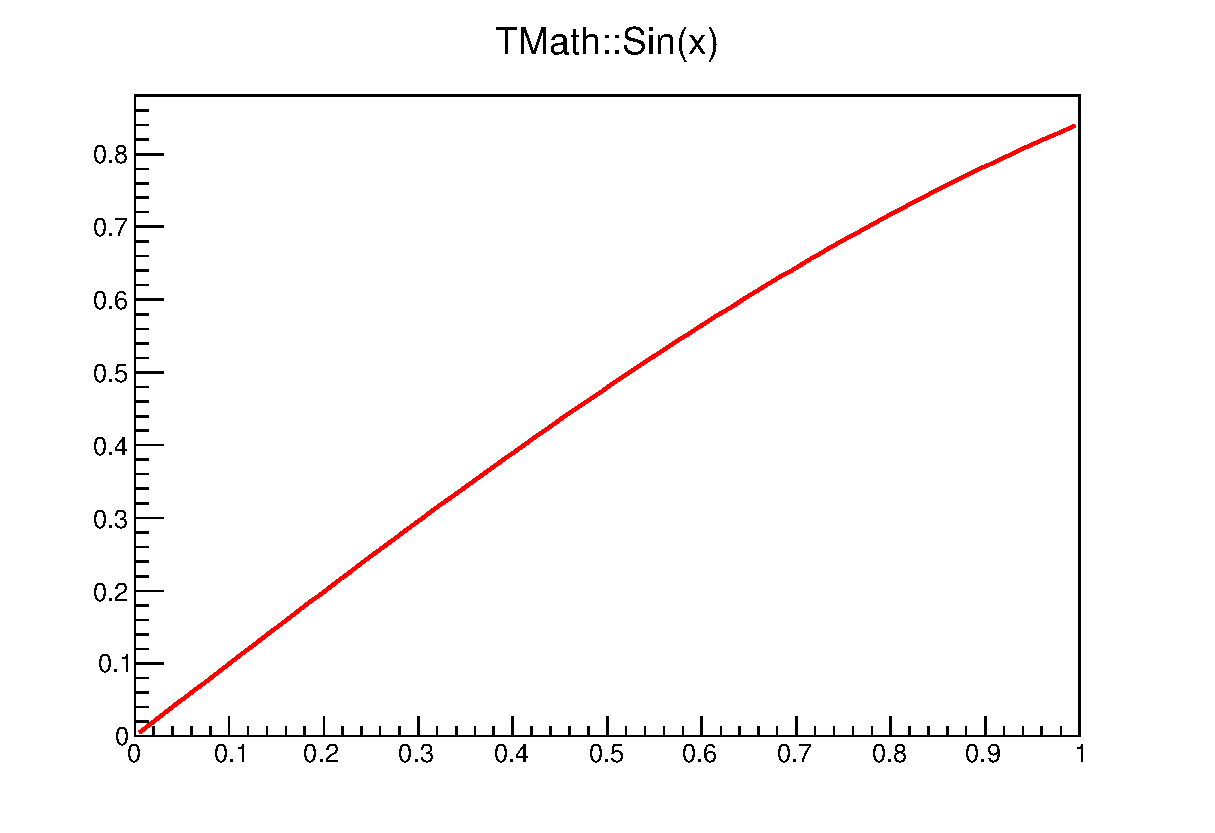
\includegraphics[width = 100mm]{./picture/sinfunctioncanvas1.eps}
 \end{center}
 \caption{\texttt{sinfunction.cpp}の実行結果}
 \label{Fig:sinfunctioncanvas1}
\end{figure}
おそらく、思っていたような定義域でない、軸に名前がついていないなどいろいろな不満があるだろう。
それらは全て人間が指定してあげる必要がある。
そういった手法も紹介していく。



これまであまりにすっ飛ばしてきたので、\verb|sinfunction.cpp|を一行目から簡単に見ていこう。
(\Cpp のお作法をしっかり学ぶつもりは無いので説明はそれなりの質なので気になる箇所は自分でググるべし)
\begin{enumerate}
 \item \verb|#include "TF1.h"| \\
       \verb|#include|とは、\Cpp のお作法であってヘッダファイル/ライブラリを読み込むということである。
       今の場合\ROOT で関数を描く為に必要となるライブラリ\verb|"TF1.h"|を読み込むという意味
 \item \verb|#include "TMath.h"| \\ 
       \ROOT で特定の定数$\pi$や$e$などの値や、
       関数$\sin(x)$、$\exp(x)$などを使用する時に必要となるライブラリ\verb|"TMath.h"|を読み込む。
 \item \verb|TF1 *sinfunction(){ |\\
       マクロの名前を準備するかを記述している箇所である。
       \Cpp では関数を定義する時に \\
       <型名> <関数名>(<引数>)\{HogeHoge\} \\
       という書き方をする。今の場合だと\\
       h       <型名> = \verb|TF1|、<関数名>=\verb|sinfunction|、<引数>=無し、といった具合である。
       \textcolor{red}{暫くの間はマクロ名とファイル名を同じにする。}
       \verb|*sinfunction|というのは\verb|sinfunction|という関数のポインタを意味するが、これ以上は触れない。
 \item \verb|TF1 *f = new TF1("f","TMath::Sin(x)") ;| \\
       ここからが\verb|sinfunction.cpp|の本文。
       この行の左辺では\verb|"TF1"|という型のポインタ\verb|f|を定義している。
       \verb|new|とは\Cpp のお作法でメモリを動的に確保する為のものである。
       \verb|TF1("f","TMath::Sin(x)")|とは左辺で定義した\verb|f|というポインタの名前を\verb|f|として、
       その間数は\verb|TMath|というライブラリの中で定義された\verb|Sin(x)|という関数にするという意味。
 \item \verb|f->Draw() ;| \\
       \verb|f|というポインタを描く。
       4行目のやり方で定義されたポインタ\verb|f|に対して命令を与える時には\verb|->|というアロー演算子を用いる。
 \item \verb|return f ;|
 \item \verb|}| \\
       3行目の\verb|{|に対応する括弧。
\end{enumerate}


  \subsection{練習}
  \begin{enumerate}
   \item 定義域を$-\pi$から$\pi$に変更せよ。
	 \begin{description}
	  \item[ヒント]  \url{http://root.cern.ch/root/html/TF1.html#TF1:TF1@1}
	 \end{description}
   \item $2\sin(x/2)$を描け。
	 \begin{description}
	  \item[ヒント]  \url{http://root.cern.ch/root/html/TF1.html#TopOfPage} の
		     B - Expression using variable x with parameters
	  \item[ヒント]\url{http://root.cern.ch/root/html/TFormula.html#TFormula:SetParameter}
	 \end{description}
   \item $ \sin(x) $と$ \cos(x) $を一緒に描け。
	 また$\sin(x)$の線を赤色、$\cos(x)$の線を緑色にせよ。
	 \begin{description}
	  \item[ヒント]  \url{http://root.cern.ch/root/html/TF1.html#TF1:Draw}
	  \item[ヒント]  \url{http://root.cern.ch/root/html/TAttLine.html#TAttLine:SetLineColor}
	 \end{description}

  \end{enumerate}

  \subsection{解答例}
  \begin{enumerate}
   \item 定義域を$ -\pi $から$ \pi $に変更せよ。
	 \begin{itembox}{\texttt{sinfunctionsol1.cpp}}
\begin{verbatim}
	...
	TF1 *sinfunctionsol1(){
	double pi = TMath::Pi() ;

	TF1 *f = new TF1("f","TMath::Sin(x)", -pi, pi) ;
	...
	}
\end{verbatim}
	 \end{itembox}

   \item $2\sin(x/2)$を描け。
	 \begin{itembox}{\texttt{sinfunctionsol2.cpp}}
\begin{verbatim}
	...
	TF1 *sinfunctionsol2(){
	double pi = TMath::Pi() ;

	TF1 *f = new TF1("f","[0]*TMath::Sin([1]*x)", -pi, pi) ;
	f->SetParameter(0, 2.) ;
	f->SetParameter(1, 0.5) ;
	...
	}
\end{verbatim}
	 \end{itembox}

   \item $\sin(x)$と$\cos(x)$を一緒に描け。
	 また$\sin(x)$の線を赤色、$\cos(x)$の線を緑色にせよ。
	 \begin{itembox}{\texttt{sinfunctionsol3.cpp}}
\begin{verbatim}
	#include "TF1.h"
	#include "TMath.h"
	TF1 *sinfunctionsol3(){
	double pi = TMath::Pi() ;

	TF1 *f = new TF1("f","TMath::Sin(x)", -pi, pi) ;
	TF1 *f2 = new TF1("f2","TMath::Cos(x)", -pi, pi) ;

	f->SetLineColor(kRed) ;
	f2->SetLineColor(kGreen) ;

	f->Draw() ;
	f2->Draw("same") ;
	return f ;
	}
\end{verbatim}
	 \end{itembox}

  \end{enumerate}
